\chapter{METODE PENELITIAN}

\section{Jenis Penelitian}
Penelitian ini mengadopsi pendekatan penelitian terapan, dengan fokus utama pada implementasi teknologi Jaringan Syaraf Tiruan dalam pengembangan sistem prediksi lama studi mahasiswa. Melalui pendekatan ini, penelitian bertujuan untuk mengaplikasikan dan mengevaluasi efektivitas metode Jaringan Syaraf Tiruan dalam konteks spesifik sistem perdiksi lama studi mahasiswa. Alur metode ini dapat dilihat pada Gambar \ref{fig:crisp-dm-overview}

\begin{figure}[H]
    \centering
    \fbox{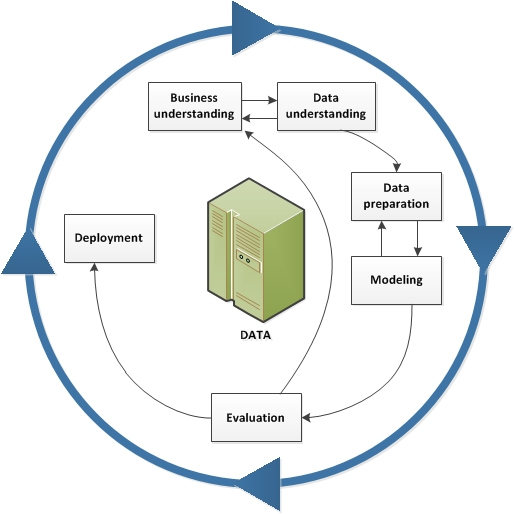
\includegraphics[width=0.55\textwidth]{images/crisp-dm-overview.jpg}}
    \caption{Alur Metode CRISP-DM \cite{IBM2022}}
    \label{fig:crisp-dm-overview}
\end{figure}

\section{Waktu dan Tempat Penelitian}
% TODO: Sesuaikan detail spesifik
Penelitian ini dilaksanakan dalam rentang waktu empat bulan, dimulai dari Agustus 2024 hingga November 2024. Pengumpulan data dilakukan melalui akuisisi dataset dari Program Studi ..., yang menyediakan basis data komprehensif mengenai data-data mahasiswa yang akan digunakan untuk membuat prediksi lama studi.

\section{Sarana dan Pendukung}
Untuk memastikan keberhasilan dan efisiensi penelitian ini, berbagai sarana pendukung telah diidentifikasi dan disiapkan. Perangkat keras dan perangkat lunak yang dipilih tidak hanya mendukung pelaksanaan penelitian, tetapi juga memungkinkan pengembangan dan pengujian sistem prediksi secara optimal. Berikut adalah rincian perangkat yang digunakan:

\subsection{Perangkat Keras}
\begin{enumerate}
    \item Memori RAM 8GB DDR3, yang menyediakan kapasitas yang memadai untuk pemrosesan data dan eksekusi model.
    \item Penyimpanan SSD 256GB, memungkinkan akses data yang cepat dan efisien, serta mempercepat proses komputasi.
\end{enumerate}

\subsection{Perangkat Lunak}
\begin{enumerate}
    \item Python versi 3 atau lebih tinggi, dipilih sebagai bahasa pemrograman utama untuk pengembangan dan implementasi model machine learning.
    \item Flask, framework web Python yang ringan dan fleksibel, digunakan untuk mengekspos model sebagai API, memfasilitasi integrasi dengan komponen sistem lainnya.
    \item Node.js, platform JavaScript server-side yang kuat, berfungsi sebagai backend untuk mengelola logika aplikasi dan alur data.
    \item React.js, library JavaScript modern untuk pengembangan antarmuka pengguna, dipilih untuk menciptakan pengalaman pengguna yang responsif dan interaktif.
    \item Figma, alat desain kolaboratif berbasis web, digunakan untuk merancang dan memprototype antarmuka pengguna sistem.
    \item Draw.io (App Diagram), platform pembuatan diagram online, dimanfaatkan untuk merancang dan mendokumentasikan arsitektur sistem melalui diagram UML.
\end{enumerate}

\section{Rancangan Penelitian}
Rancangan penelitian ini disusun secara sistematis untuk memastikan pelaksanaan yang terstruktur dan efektif. Dengan mengadopsi metodologi Cross-Industry Standard Process for Data Mining (CRISP-DM), penelitian ini dibagi menjadi beberapa tahapan kritis yang saling terkait. Setiap tahapan dirancang untuk membangun fondasi bagi tahapan berikutnya, memastikan kesinambungan dalam proses penelitian. Berikut adalah uraian detail dari setiap tahapan:

\subsection{Business Understanding}
Tahap ini berfokus pada pemahaman mendalam tentang kebutuhan dan tantangan dalam memprediksi lama studi mahasiswa di institusi pendidikan tinggi. Melalui wawancara dengan stakeholder akademik seperti dosen pembimbing. Tujuan spesifik dari sistem prediksi yang akan dikembangkan menggunakan Jaringan Syaraf Tiruan akan didefinisikan dengan jelas. Pemahaman ini akan menjadi landasan untuk merancang solusi prediksi yang akurat, tepat sasaran, dan bernilai tinggi bagi institusi dalam upaya meningkatkan tingkat kelulusan tepat waktu dan mengurangi angka putus kuliah.

\subsection{Data Understanding}
Pada tahap ini, peneliti akan melakukan eksplorasi mendalam terhadap dataset akademik mahasiswa yang tersedia. Aktivitas ini mencakup analisis statistik deskriptif, visualisasi data, dan identifikasi pola yang mungkin mempengaruhi lama studi mahasiswa. Dataset yang akan dieksplorasi meliputi data akademik seperti IPK per semester, nilai mata kuliah, data demografis mahasiswa. Pemahaman yang baik tentang karakteristik data, termasuk kualitas, kelengkapan, dan relevansinya terhadap prediksi lama studi, akan membantu dalam merancang strategi preprocessing yang efektif dan pemilihan fitur yang tepat untuk model Jaringan Syaraf Tiruan. Analisis korelasi antar variabel juga akan dilakukan untuk mengidentifikasi faktor-faktor yang memiliki pengaruh signifikan terhadap lama studi mahasiswa.

\subsection{Data Preparation}
Tahap persiapan data melibatkan serangkaian proses untuk mengolah data akademik mahasiswa menjadi format yang siap digunakan dalam pemodelan Jaringan Syaraf Tiruan. Kegiatan ini mencakup pembersihan data untuk mengatasi nilai yang hilang atau tidak konsisten pada record akademik, normalisasi atau standarisasi fitur numerik seperti IPK dan nilai mata kuliah, encoding variabel kategorikal seperti jurusan atau status mahasiswa, dan potentially feature engineering untuk menciptakan fitur baru yang lebih informatif, misalnya rata-rata nilai mata kuliah inti. Selain itu, dataset akan dibagi menjadi set pelatihan dan pengujian untuk memfasilitasi evaluasi model prediksi lama studi yang akurat.

\subsection{Modeling}
Dalam tahap pemodelan, peneliti akan mengimplementasikan metode Jaringan Syaraf Tiruan dengan algoritma backpropagation untuk memprediksi lama studi mahasiswa. Proses ini melibatkan eksperimen dengan berbagai arsitektur jaringan, penentuan jumlah layer dan neuron yang optimal, serta tuning hyperparameter seperti learning rate dan momentum. Validasi silang akan digunakan untuk mengoptimalkan performa model. Fokus utama adalah pada pengembangan model JST yang dapat menangkap kompleksitas hubungan antara berbagai faktor akademik dan non-akademik yang mempengaruhi lama studi mahasiswa.

\subsection{Evaluation}
Evaluasi model JST akan dilakukan secara komprehensif menggunakan berbagai metrik kinerja seperti Mean Absolute Error (MAE), Root Mean Square Error (RMSE), dan koefisien determinasi (R²) untuk mengukur akurasi prediksi lama studi. Selain itu, analisis sensitivitas akan dilakukan untuk memahami pengaruh relatif dari berbagai input terhadap prediksi. Proses evaluasi ini juga akan mencakup perbandingan dengan metode machine learning lainnya seperti regresi linear dan decision tree untuk mengukur keunggulan pendekatan JST dalam konteks prediksi lama studi mahasiswa.

\subsection{Deployment}
Setelah model JST final dipilih dan divalidasi, tahap deployment akan fokus pada integrasi model ke dalam sistem informasi akademik yang ada di institusi. Ini melibatkan pengembangan antarmuka pengguna yang user-friendly untuk staf akademik, implementasi backend untuk menjalankan prediksi, dan penyiapan API untuk mengintegrasikan fungsionalitas prediksi dengan sistem yang ada. 

\subsection{Feedback}
Tahap akhir penelitian akan melibatkan pengumpulan dan analisis umpan balik dari pengguna sistem prediksi lama studi. Melalui survei pengguna, analisis akurasi prediksi terhadap hasil aktual, dan wawancara dengan stakeholder, peneliti akan mengidentifikasi area untuk perbaikan dan pengembangan lebih lanjut. Informasi ini akan digunakan untuk merumuskan rekomendasi untuk iterasi dan peningkatan sistem di masa depan, memastikan bahwa sistem prediksi lama studi menggunakan JST terus berkembang sesuai dengan dinamika akademik dan kebutuhan institusi pendidikan tinggi.

\section{Jadwal Penelitian}
Jadwal dan waktu pelaksanaan penelitian ini dapat dilihat pada Tabel \ref{tab:jadwal-penelitian}. 

\begin{table}[htbp]
    \centering
    \setlength{\tabcolsep}{4pt}
    \renewcommand{\arraystretch}{1.2}
    \caption{Jadwal Kegiatan Penelitian}
    \label{tab:jadwal-penelitian}
    \begin{tabular}{|c|p{4cm}|c|c|c|c|}
    \hline
    \multirow{2}{*}{\textbf{No}} & \multirow{2}{*}{\textbf{Kegiatan}} & \multicolumn{4}{c|}{\textbf{Bulan}} \\
    \cline{3-6}
     & & \textbf{Agustus} & \textbf{September} & \textbf{Oktober} & \textbf{November} \\
    \hline
    1. & Studi pustaka & \cellcolor{lightgray} & & & \\
    \hline
    2. & Penerimaan proposal & \cellcolor{lightgray} & \cellcolor{lightgray} & & \\
    \hline
    3. & Pengumpulan dan analisis data & \cellcolor{lightgray} & \cellcolor{lightgray} & & \\
    \hline
    4. & Pembuatan sistem & & \cellcolor{lightgray} & \cellcolor{lightgray} & \\
    \hline
    5. & Pengujian hasil & & & \cellcolor{lightgray} & \\
    \hline
    6. & Penyelesaian laporan dan aplikasi akhir & & & \cellcolor{lightgray} & \cellcolor{lightgray} \\
    \hline
    \end{tabular}
\end{table}


